\documentclass[unknownkeysallowed]{beamer}
\usetheme{Madrid}
\usepackage{subfig}
\usepackage{xcolor}
\usepackage{wrapfig}
\usepackage[utf8]{inputenc}
\usepackage[polish]{babel}
\usepackage[T1]{fontenc}

\title{Gradient Naturalny}
\subtitle{}
\author{Jakub Bartczuk}
\centering
\date{Kwiecień 2020}
\begin{document}
\maketitle

% macros
\newcommand{\gradfx}{\nabla f(x)}

\begin{frame}{Gradient Descent}
  Minimalizujemy różniczkowalną funkcję $f$.

  Przybliżenie szeregiem Taylora pierwszego rzędu daje
  $$f(x + \delta) \approx g(x) = f(x) + \gradfx^T \delta $$

  Minimalizacja g sugeruje procedurę 
  $$x_{t+1} = x_t - \alpha \nabla f(x_t)$$

  $\alpha$ znajdujemy line searchem

\end{frame}

\begin{frame}{Problemy z GD}
  Metoda nie jest niezmiennicza względem reparametryzacji: zbieżność zależy od wartości własnych Hesjanu
    \begin{columns}

        \column{.5\textwidth}
        \begin{center}$f(x,y ) = x^2 + y^2$\end{center}
        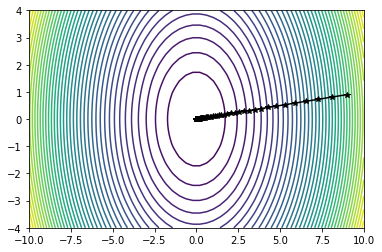
\includegraphics[width=\textwidth]{GD1.png} 
        \column{.5\textwidth}
        \begin{center}$f(x,y ) = x^2 + 10 y^2$\end{center}
        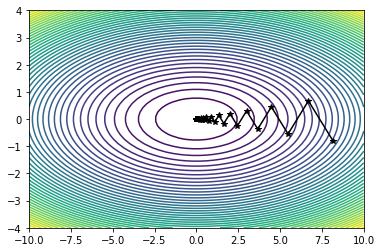
\includegraphics[width=\textwidth]{GD10.png} 
    \end{columns}
\end{frame}

\begin{frame}{Metody Spadku (Steepest descent)}
  Powyższą procedurę można zinterpretować tak: dla zadanej normy $\| \|$

  $$\Delta x_{nsd} = argmin_v \{\gradfx v : \|v\| = 1 \}$$ 
  $$f(x + \delta) \approx g(x) = f(x) + \gradfx^T \delta $$
  
  Szukanie $\Delta x_{nsd}$ z różnych norm $\|x\| = \|Px\|_2$ jest równoważne optymalizacji spadkiem gradientu funkcji $h(x) = f(P^{1/2}x)$ \pause
  

  Intuicyjne jest żeby zmienić parametryzację tak, aby uwarunkowanie Hesjanu było równe 1.
  \begin{block}{Metoda Newtona}
  $$x_{t+1} = x_t - H_f(x)^{-1} \nabla f(x_t)$$
  \end{block}

\end{frame}

\begin{frame}{Wypukłość}
  Powyższe metody zakładały wypukłość 

  Przykład: Hesjan który nie jest dodatnio określony (start w punkcie siodłowym)

 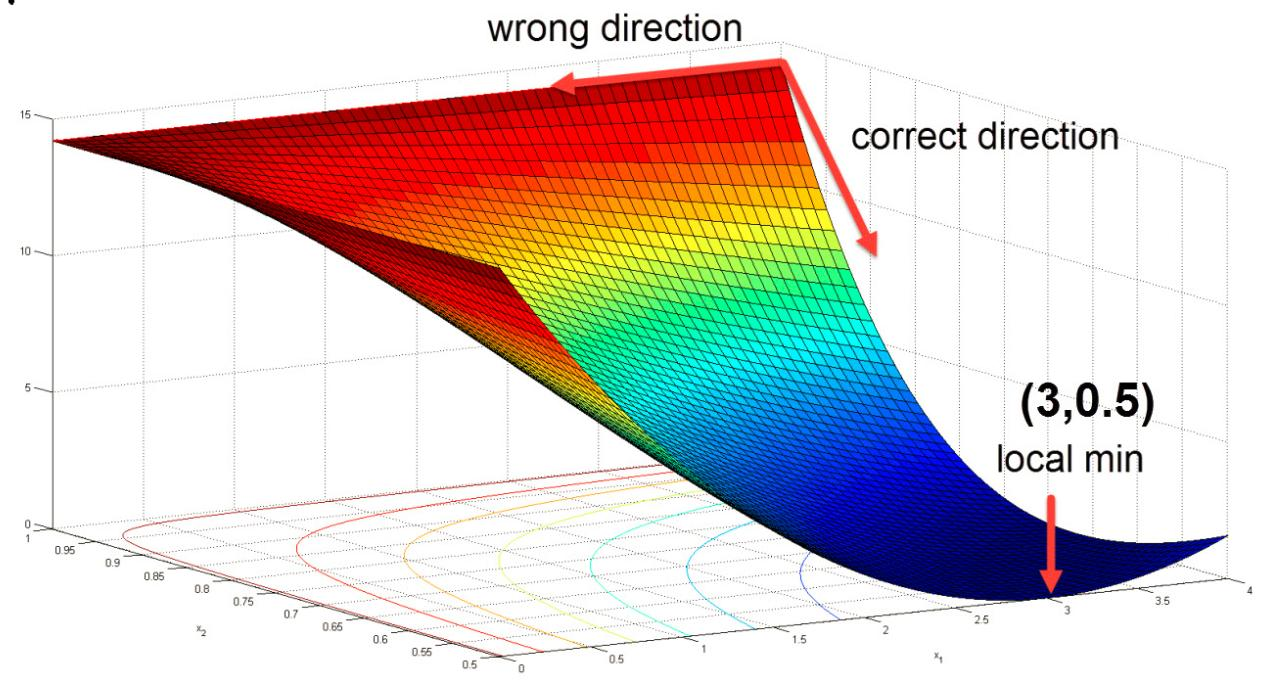
\includegraphics[width=\textwidth]{Niewypukla.jpg} 
\end{frame}

\begin{frame}{Co wspólnego mają powyższe metody}
  \begin{block}{Metody spadku}
  Zakładamy, że $\delta$ jest małe tzn $\| \delta \| < \epsilon$
  Przybliżamy $f(x + \delta)$
  \end{block}

  \begin{block}{Gradient naturalny}
    $\theta$ parametryzuje rodzinę rozkładów $p_{\theta}$

    $J(\theta) = \mathbb{E}_{x \sim p_{\theta}}[c(x)]$

    Minimalizujemy $J(\theta)$ za pomocą $p_{\theta + \delta}$ bliskiego w sensie KL-dywergencji
  \end{block}

\end{frame}


\begin{frame}{Gradient Naturalny}
  \begin{block}{GN dokładniej}
  Szukamy $\delta$ takiego, że $KL(p_{\theta + \delta} || p_{\theta}) < \epsilon$
  $$argmin_{\delta} J(\theta + \delta) \approx g(\theta) = J(\theta) + \nabla J(\theta)^T \delta $$
  \end{block}

  \end{frame}



\end{document}